\tsDef{Separation of Variables}{
The method of separation of variables is particularly suitable for
differential equations of the form
\(
y'(x)=f(x)\cdot g(y).
\)
The idea is to move all terms involving the independent variable
to one side and all terms involving the dependent variable to the
other side, and then integrate both sides.
}
\\
\tsDef{Linear Substitution}{
A differential equation of the form
\[
\frac{dy}{dx}=y' = f(ax+by+c),
\qquad a,b,c\in\mathbb R,
\]
can be transformed into a differential equation with separable
variables by the substitution:
\(
u=ax+by+c.
\)
}
\\
\tsIdea{Autonomous Equation}{
After the substitution
\(
u=ax+by+c,
\)
the differential equation
\(
\frac{dy}{dx}=f(ax+by+c)
\)
becomes
\[
\frac{du}{dx}
=
a+b\frac{dy}{dx}
=
a+bf(u).
\]
The independent variable $x$ no longer appears explicitly on the
right-hand side. Such a differential equation is called
\emph{autonomous}.
}
\tsDef{Homogeneous Differential Equation}{
A differential equation of the form
\[
\frac{dy}{dx}
=
g\!\left(\frac{y}{x}\right)
\]
is called \emph{homogeneous in the variables}. It can be transformed into a differential equation with separable
variables by the substitution
\(
u=\frac{y}{x}.
\)
}
\tsDef{Associated Homogeneous Equation}{
Given an inhomogeneous differential equation
\[
a_n(x)y^{(n)}(x)+\cdots+a_0(x)y(x)=s(x),
\qquad s(x)\neq 0,
\]
the equation
\(
a_n(x)y^{(n)}(x)+\cdots+a_0(x)y(x)=0
\)
is called the associated homogeneous differential equation.
}
\\
\tsThe{General Solution of a Linear Inhomogeneous ODE}{
Let
\(
y_p(x)
\)
be a particular solution of a linear inhomogeneous differential
equation and let
\(
y_h(x)
\)
be the general solution of the associated homogeneous equation.Then
\(
y(x)=y_h(x)+y_p(x)
\)
is the general solution of the linear inhomogeneous differential
equation.
}
\\
\tsDef{Variation of Constants}{
Consider a first-order linear inhomogeneous differential equation. A particular solution can be obtained by replacing the constant
appearing in the general solution of the associated homogeneous
equation by a function of the independent variable. This method is called \emph{variation of constants}.
}
\\
\tsEx{Variation of Constants Example}{
Given
\[
y'-y=x,
\]
the associated homogeneous equation
\[
y'-y=0
\]
has general solution
\[
y_h(x)=Ke^x.
\]
The variation-of-constants ansatz is therefore
\[
y_p(x)=K(x)e^x.
\]
}
\tsThe{Standard Ans\"atze for Particular Solutions}{
For a linear inhomogeneous ODE $L(y)=s(t)$:
\[
\begin{array}{|c|c|}
\hline
\textbf{Forcing term } s(t) & \textbf{Ansatz } y_p(t)\\
\hline
a_0+a_1t+\cdots+a_nt^n
&
C_0+C_1t+\cdots+C_nt^n
\\
\hline
Ae^{kt}
&
Ce^{kt}
\\
\hline
A\sin(\omega t)+B\cos(\omega t)
&
C_1\sin(\omega t)+C_2\cos(\omega t)
\\
\hline
\end{array}
\]
If the corresponding characteristic root has multiplicity $m$, multiply the ansatz by $t^m$. That is:
\(
0 \leadsto t^m, \
k \leadsto t^m, \
i\omega \leadsto t^m.
\)
}
\\
\tsThe{Picard--Lindel\"of--Peano (First Order)}{
The initial value problem
\[
y'=f(x,y),
\qquad
y(x_0)=y_0,
\]
has, for sufficiently well-behaved functions $f$, a unique solution
\(
x\mapsto y(x),\ x\in I,
\)
where the interval $I$ may depend on $x_0$ and $y_0$. 
}
\tsThe{Picard--Lindel\"of--Peano (Higher Order)}{
The initial value problem
\[
y^{(n)}
+f_{n-1}(x)y^{(n-1)}
+\cdots
+f_1(x)y'
+f_0(x)y
=
s(x),
\]
with initial conditions
\[
y(x_0)=y_0,
\qquad
y'(x_0)=v_0,
\qquad
\dots,
\qquad
y^{(n-1)}(x_0)=z_0,
\]
has, for sufficiently well-behaved functions
\(
f_{n-1},\dots,f_0,s,
\)
a unique solution
\(
x\mapsto y(x),
\ x\in I,
\)
where the interval $I$ may depend on $x_0$ and the prescribed
initial data.
}
\\

% Preamble:
% \usepackage{tikz}
% \usetikzlibrary{arrows.meta,positioning,calc}

\begin{center}
\resizebox{0.35\textwidth}{!}{%
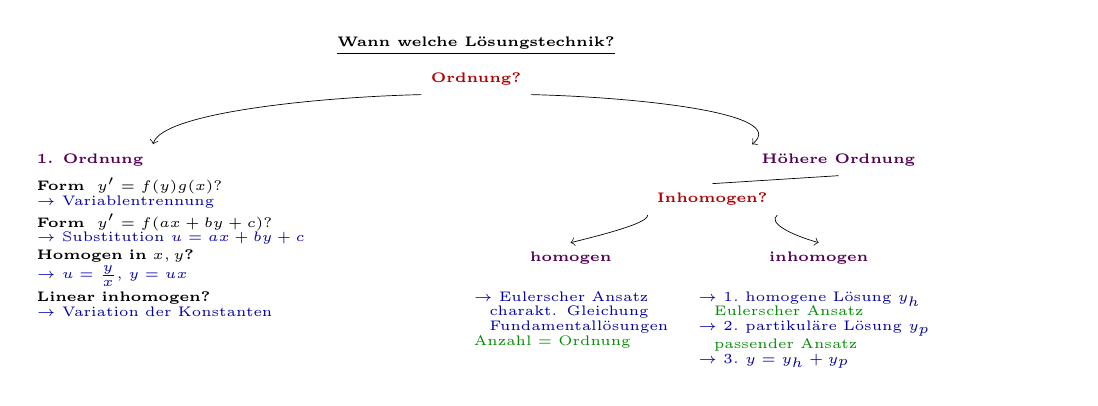
\begin{tikzpicture}[
    font=\fontsize{5}{5.3}\selectfont,
    line width=0.25pt,
    title/.style={align=center},
    question/.style={align=center,text=red!70!black},
    heading/.style={align=left,text=violet!65!black},
    method/.style={align=left,text=blue!65!black},
    body/.style={align=left}
]

\node[title] (title) at (0,0)
    {\underline{\textbf{Wann welche Lösungstechnik?}}};

\node[question] (order) at (0,-0.42)
    {\textbf{Ordnung?}};

% Left branch
\node[heading,anchor=north west] (first) at (-5.7,-1.25)
    {\textbf{1. Ordnung}};

\draw[->]
    (order.south west)
    .. controls (-2.0,-0.65) and (-4.0,-0.85) ..
    (first.north east);

\node[body,anchor=north west,text width=5.2cm]
    at (-5.7,-1.55)
{
\textbf{Form } $y'=f(y)g(x)$?

{\color{blue!65!black}
$\rightarrow$ Variablentrennung}

\vspace{0.4mm}

\textbf{Form } $y'=f(ax+by+c)$?

{\color{blue!65!black}
$\rightarrow$ Substitution $u=ax+by+c$}

\vspace{0.4mm}

\textbf{Homogen in $x,y$?}

{\color{blue!65!black}
$\rightarrow$ $u=\frac{y}{x}$, $y=ux$}

\vspace{0.4mm}

\textbf{Linear inhomogen?}

{\color{blue!65!black}
$\rightarrow$ Variation der Konstanten}
};

% Right branch
\node[heading,anchor=north east] (higher) at (5.7,-1.25)
    {\textbf{Höhere Ordnung}};

\draw[->]
    (order.south east)
    .. controls (2.0,-0.65) and (4.0,-0.85) ..
    (higher.north west);

\node[question] (inhom) at (3.0,-1.95)
    {\textbf{Inhomogen?}};

\draw (higher.south) -- (inhom.north);

\node[heading] (homogeneous) at (1.2,-2.7)
    {\textbf{homogen}};

\draw[->]
    (inhom.south west)
    .. controls (2.2,-2.25) and (1.6,-2.4) ..
    (homogeneous.north);

\node[method,anchor=north west,text width=3.8cm]
    at (-0.15,-3.0)
{
$\rightarrow$ Eulerscher Ansatz

\hspace{2mm}charakt. Gleichung

\hspace{2mm}Fundamentallösungen

{\color{green!55!black}
Anzahl = Ordnung}
};

\node[heading] (inhomogeneous) at (4.35,-2.7)
    {\textbf{inhomogen}};

\draw[->]
    (inhom.south east)
    .. controls (3.7,-2.25) and (4.0,-2.4) ..
    (inhomogeneous.north);

\node[method,anchor=north west,text width=4.6cm]
    at (2.7,-3.0)
{
$\rightarrow$ $1.$ homogene Lösung $y_h$

{\color{green!55!black}
\hspace{2mm}Eulerscher Ansatz}

$\rightarrow$ $2.$ partikuläre Lösung $y_p$

{\color{green!55!black}
\hspace{2mm}passender Ansatz}

$\rightarrow$ $3.$ $y=y_h+y_p$
};

\end{tikzpicture}%
}
\end{center}